\documentclass[11pt]{article}
\usepackage[margin=2.5cm]{geometry}
\usepackage{amsmath,amssymb,graphicx,booktabs,hyperref,float}
\usepackage[T1]{fontenc}
\setlength{\parskip}{4pt}
\graphicspath{{figures/}}

\title{Real-Time PM2.5 Stream Intelligence for Astana\\\large Real-Time Data Analysis --- Endterm Project}
\author{Yerlan Utepbergenov\\Group BDA-2401\\\small Code: \url{https://github.com/utepbergenoff/realtime_data}}
\date{November 2026}

\begin{document}
\maketitle

\begin{abstract}
This project extends a simple streaming application into an intelligent air-quality monitoring system for four districts of Astana. A reproducible generator produces 1-minute PM2.5 readings with daily seasonality, a trend, weather effects, correlated noise and labelled anomalies. A producer partitions the stream by sensor key into queues, and a pool of consumer workers processes every event online: it detects anomalies with a rolling median/MAD detector and a rolling z-score, and forecasts PM2.5 five minutes ahead with an online SGD regressor trained test-then-train. A live dashboard shows the stream, forecasts, anomaly counts, throughput and backlog while data arrives. Time-series analysis recovers the built-in seasonality and trend. The MAD detector reaches recall 1.00 and F1 0.88 (z-score: F1 0.36), the forecaster beats the persistence baseline by 5.3\% MAE on normal points, and the pipeline sustains 1{,}495 events/s with a median latency of 2.9 ms.
\end{abstract}

\section{Introduction and Objective}
Fine particulate matter (PM2.5) is one of the main air-quality problems in Astana in winter, when heating and traffic add to cold, still air. A city monitoring network produces a continuous stream of sensor readings. Its value is in reacting \emph{while} the data arrives: showing the current situation, raising an alert when a reading is abnormal, and anticipating the next minutes.

Assignment~3 detected anomalies in 14 points from a single sensor. The goal of this endterm project is to turn that into a complete streaming system that covers the four topics of weeks 5--8:
\begin{enumerate}\itemsep0pt
\item \textbf{Real-time visualization}: a dashboard with several views that updates continuously while the stream runs.
\item \textbf{Time-series analysis}: timestamps, resampling, rolling windows, trend and daily seasonality.
\item \textbf{Anomaly detection and real-time ML}: an online detector and an online 5-minute-ahead forecaster, both evaluated with proper metrics and using only information available at prediction time.
\item \textbf{Distributed stream processing}: a producer, key-partitioned streams and multiple consumer workers, with measured operational characteristics (throughput, latency, backlog, events per worker).
\end{enumerate}
Table~\ref{tab:req} maps each requirement of the task to the part of the implementation that covers it.

\begin{table}[H]
\centering\small
\begin{tabular}{@{}ll@{}}
\toprule
Requirement & Where it is covered \\
\midrule
Continuously updated visualization ($\ge$2 views) & Live 4-panel dashboard (Section~\ref{sec:dash}) \\
Time-series analysis & Resampling, rolling windows, decomposition (Section~\ref{sec:ts}) \\
Anomaly detection + evaluation & Rolling MAD and z-score; precision/recall/F1 (Section~\ref{sec:anom}) \\
Real-time ML component & Online SGD forecaster, $t+5$ min (Section~\ref{sec:ml}) \\
Features available at prediction time & Causal features, test-then-train (Section~\ref{sec:ml}) \\
ML evaluation (MAE/RMSE) & Against a persistence baseline (Section~\ref{sec:ml}) \\
Distributed stream processing & Producer, partitions, worker pool (Section~\ref{sec:arch}) \\
$\ge$2 operational characteristics & Throughput, latency, backlog, events/worker (Section~\ref{sec:ops}) \\
\bottomrule
\end{tabular}
\caption{Task requirements and where they are implemented.}
\label{tab:req}
\end{table}

\section{Related Work and Background}
\textbf{Stream processing.} Apache Kafka \cite{kafka} stores a stream as a topic split into partitions. A record's key decides its partition, ordering is guaranteed only within a partition, and each partition is read by exactly one consumer of a consumer group. Spark Structured Streaming \cite{spark} and Apache Flink \cite{flink} process such streams with keyed operators that keep per-key state and run in parallel on many machines. This project reproduces these concepts on one machine with Python threads and queues: the partitioning, the one-consumer-per-partition rule and the per-key state are the same, only the transport is simulated.

\textbf{Anomaly detection.} The classic z-score compares a value with the mean and standard deviation of a reference window. Both statistics are sensitive to outliers, so an anomaly can hide the anomalies that follow it (\emph{masking}). Leys et al.\ \cite{leys} recommend the median absolute deviation (MAD) instead, because the median has a breakdown point of 50\%.

\textbf{Online learning.} Data streams require models that update incrementally and can follow changes in the data (\emph{concept drift}) \cite{gama}. Stochastic gradient descent, available in scikit-learn \cite{sklearn} through \texttt{partial\_fit}, updates a linear model one mini-batch at a time. For evaluation, the prequential (test-then-train) scheme \cite{dawid} uses each example first to test the model and then to train it, so every reported error is out-of-sample.

\section{Data Generation}
Real sensor data has no ground truth for anomalies, so a synthetic generator is used. Every series is built from known parts, so every result can be checked against the truth. The generator produces 1-minute readings for 4 districts (Yesil, Almaty, Saryarka, Baikonur) over 3 days, which gives $3\times1440\times4=17{,}280$ events. For sensor $i$ at minute $t$ with hour of day $h$:
\begin{equation}
\text{pm}_t = b_i + \underbrace{10\,e^{-((h-8)/2)^2} + 14\,e^{-((h-19)/2.5)^2}}_{\text{daily seasonality}} + \underbrace{3\,d_t}_{\text{trend}} - 1.5\,(w_t-4) + a_t + \varepsilon_t,
\end{equation}
where $b_i = 25+5i$ is the district level, $d_t$ is time in days, $w_t$ is wind speed (stronger wind disperses pollution), $a_t = 0.95\,a_{t-1} + \mathcal N(0,0.6^2)$ is AR(1) correlated noise and $\varepsilon_t\sim\mathcal N(0,1)$ is white sensor noise. The two Gaussian bumps model the morning traffic peak (08:00) and the larger evening peak (19:00, traffic plus heating). Temperature follows a daily sine wave around $-8\,^\circ$C.

Two kinds of labelled anomalies are injected per sensor: 6 \emph{pollution spikes} (+50 to +100\,$\mu$g/m$^3$ for 5--15 minutes) and 2 \emph{sensor dropouts} (readings near 0 for 3--7 minutes). In total there are 223 spike minutes and 40 dropout minutes (1.5\% of the data). The labels \texttt{is\_anomaly} and \texttt{anomaly\_type} are removed from the events before streaming. They are joined back only for evaluation, so the detectors never see them. All parameters are stored in one \texttt{CONFIG} dictionary, which is saved to \texttt{config.json}. With \texttt{seed = 42} the dataset is identical on every run. Figure~\ref{fig:stream} shows the generated stream.

\begin{figure}[H]
\centering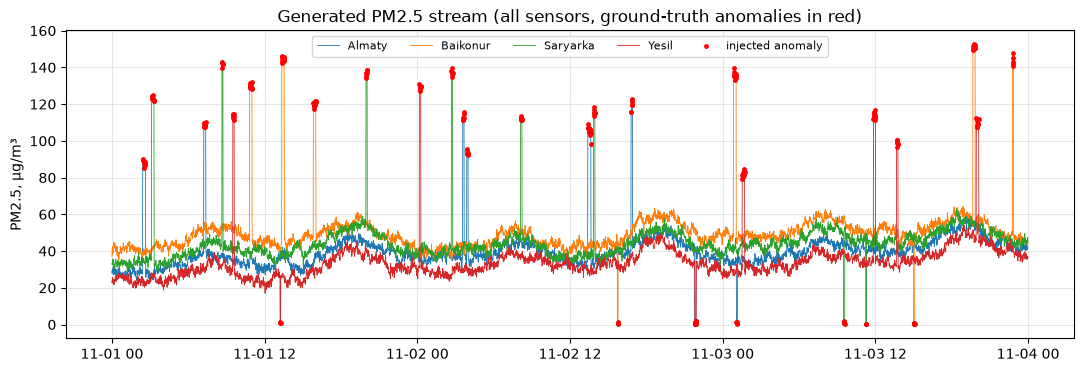
\includegraphics[width=0.9\linewidth]{stream.png}
\caption{Generated PM2.5 stream for all sensors. Injected anomalies (ground truth) are shown in red.}
\label{fig:stream}
\end{figure}

\section{System Architecture and Stream Processing}
\label{sec:arch}
{\footnotesize
\begin{verbatim}
generator --> producer --> partition queues --> worker pool --> results queue --> sink
(CSV, time   (key =       crc32(key) % N      (N threads,                     (main thread:
 ordered)     sensor_id)                        per-sensor state)              dashboard)
\end{verbatim}
}

\textbf{Producer.} The producer replays the events in timestamp order. A rate limiter keeps the replay at 1{,}500 events/s to simulate a live feed. Each event is stamped with \texttt{t\_ingest} and routed to partition $\text{crc32}(\text{sensor\_id}) \bmod N$. A stable hash is required: Python's built-in \texttt{hash()} of a string is randomised per process, so the same sensor could land in a different partition on every run. CRC32 always maps the same key to the same partition. With $N=2$, partition 0 holds Yesil and Baikonur and partition 1 holds Almaty and Saryarka.

\textbf{Partitions and workers.} Each partition is a thread-safe \texttt{queue.Queue}, read by exactly one worker thread. Because all events of a sensor go to one partition and one worker, \textbf{per-sensor order is preserved}, and the worker can keep that sensor's state (rolling window, pending forecasts) in local memory without locks. This is the same design as a Kafka consumer group or a Flink keyed stream. For every event the worker runs anomaly detection (Section~\ref{sec:anom}) and the forecaster (Section~\ref{sec:ml}), stamps \texttt{t\_done} and sends the result to a results queue.

\textbf{Sink.} The main thread drains the results queue, samples the backlog (events waiting in all partition queues) and redraws the dashboard. When the producer has sent the last event, it puts an end-of-stream marker into every partition so that the workers stop cleanly.

\section{Real-Time Visualization}
\label{sec:dash}
While the producer and the workers run in background threads, the sink redraws a 4-panel dashboard every 1.5 seconds (Figure~\ref{fig:dash}):
\begin{enumerate}\itemsep0pt
\item \textbf{Live PM2.5} for one district over the last 3 hours of stream time, with the 5-minute-ahead forecast and the detected anomalies.
\item \textbf{Anomalies detected per district}, as a running count.
\item \textbf{Throughput and backlog} over wall-clock time.
\item \textbf{KPI panel}: events processed, average throughput, latency p50/p95, current backlog, number of anomalies and the live forecast MAE.
\end{enumerate}
Each view answers a different operational question: what is happening now, where the problems are, and whether the system keeps up.

\begin{figure}[H]
\centering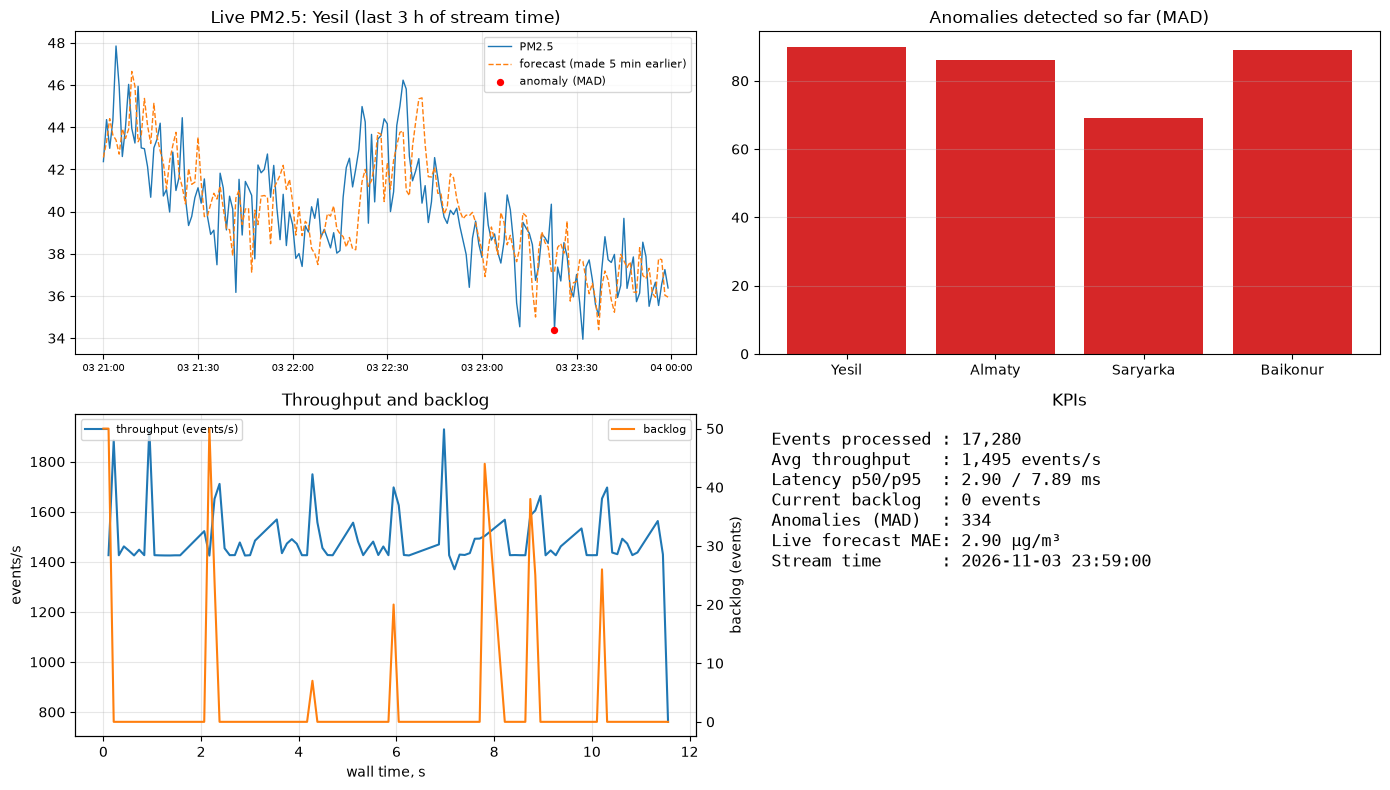
\includegraphics[width=\linewidth]{dashboard.png}
\caption{Live dashboard (final frame). Top: live PM2.5 with forecast and anomaly flags; anomaly counts per district. Bottom: throughput and backlog; KPI panel.}
\label{fig:dash}
\end{figure}

\section{Time-Series Analysis}
\label{sec:ts}
The processed stream is indexed by timestamp and analysed with three temporal methods:
\begin{itemize}\itemsep0pt
\item \textbf{Resampling} from 1-minute to 15-minute and hourly medians. Resampling aggregates fixed, non-overlapping buckets and reduces the number of points. The median is used so that anomalies do not distort the result.
\item \textbf{Rolling windows} of 1 hour (mean and median) and 24 hours (mean). A rolling window slides over every point and keeps the original frequency (Figure~\ref{fig:rolling}).
\item \textbf{Decomposition} of the hourly median series into trend, daily seasonality and residual. The trend is a centred 24-hour moving average (one full daily cycle, so the seasonality averages out). The seasonal component is the mean detrended value for each hour of the day, and the residual is what remains.
\end{itemize}

\begin{figure}[H]
\centering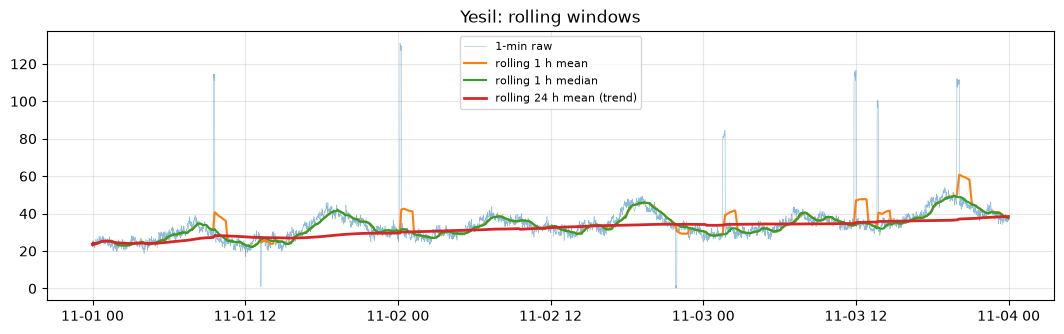
\includegraphics[width=0.85\linewidth]{rolling.png}
\caption{Yesil: raw 1-minute readings with 1-hour and 24-hour rolling windows.}
\label{fig:rolling}
\end{figure}

\begin{figure}[H]
\centering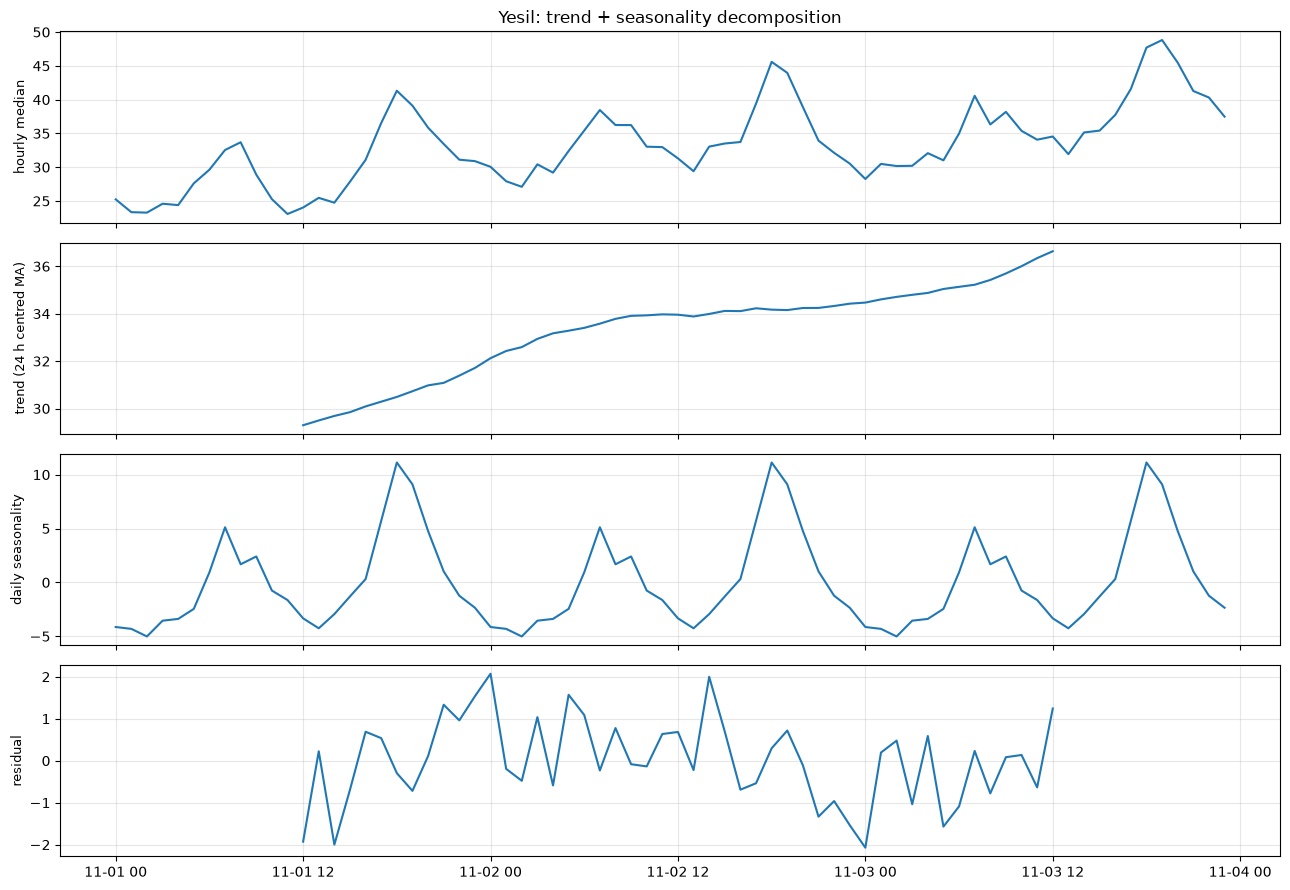
\includegraphics[width=0.75\linewidth]{decomposition.png}
\caption{Yesil: decomposition of the hourly median into trend, daily seasonality and residual.}
\label{fig:decomp}
\end{figure}

\textbf{Findings.} The decomposition (Figure~\ref{fig:decomp}) recovers the structure that was built into the generator:
\begin{itemize}\itemsep0pt
\item \textbf{Daily seasonality}: a morning peak at 07:00, a larger evening peak at 18:00 (+11.1\,$\mu$g/m$^3$ above trend) and a minimum at 02:00. Figure~\ref{fig:profile} shows the same shape in every district.
\item \textbf{Trend}: the 24-hour rolling mean rises by 3.67\,$\mu$g/m$^3$ per day (true value: +3.0). The difference comes from the wind cycle (period 1.7 days), which a 24-hour window cannot fully average out.
\item \textbf{Residual}: after removing trend and seasonality, the standard deviation drops from 5.97 to 1.01, so these two components explain most of the hourly variation.
\item District levels differ (Yesil lowest, Baikonur highest), but the daily shape is the same, so one seasonal model could be shared across sensors.
\end{itemize}

\begin{figure}[H]
\centering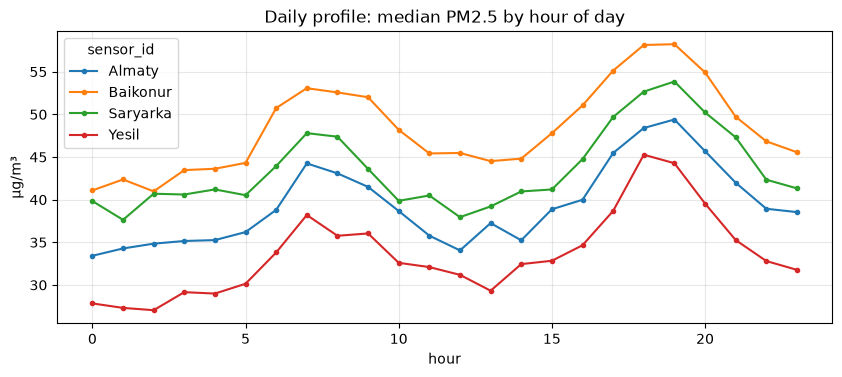
\includegraphics[width=0.65\linewidth]{daily_profile.png}
\caption{Daily profile: median PM2.5 by hour of day for each district.}
\label{fig:profile}
\end{figure}

\section{Anomaly Detection}
\label{sec:anom}
\subsection{Method}
Each worker keeps, per sensor, a window of the \textbf{previous 30 values}. A new value $x$ is scored against this window \emph{before} it is added, so an anomaly cannot inflate the statistics it is tested against. Scoring starts after 15 values of history. Two detectors are compared:
\begin{align}
\text{MAD score} &= \frac{|x-\operatorname{median}(W)|}{1.4826\cdot\operatorname{MAD}(W)}, \qquad \operatorname{MAD}(W)=\operatorname{median}\big(|W-\operatorname{median}(W)|\big), \\
\text{z-score} &= \frac{|x-\bar W|}{s_W}.
\end{align}
The constant 1.4826 makes the MAD comparable to the standard deviation for normal data. Both denominators have a floor of 0.5 to avoid division by zero on flat windows. A minute is flagged if the MAD score exceeds $k=4$, or if the z-score exceeds $k=3$. The detector is fully causal and runs in constant time per event.

\subsection{Evaluation}
The online flags are compared with the injected ground truth at two levels: per minute (precision, recall, F1) and per episode. An episode counts as detected if any of its minutes is flagged, and the detection delay is measured from the episode start. Accuracy is not used: 98.5\% of minutes are normal, so a detector that never fires would score 98.5\%.

\begin{table}[H]
\centering\small
\begin{tabular}{@{}lccccc@{}}
\toprule
Method & Precision & Recall & F1 & Flags & False positives \\
\midrule
Rolling MAD ($k=4$) & \textbf{0.787} & \textbf{1.000} & \textbf{0.881} & 334 & 71 \\
Rolling z-score ($k=3$) & 0.347 & 0.365 & 0.356 & 277 & 181 \\
\bottomrule
\end{tabular}
\caption{Point-level anomaly detection results (17{,}280 minutes, 263 anomalous).}
\label{tab:anom}
\end{table}

\begin{table}[H]
\centering\small
\begin{tabular}{@{}llcccc@{}}
\toprule
Method & Type & Episodes & Detected & Mean delay (min) & Share of minutes flagged \\
\midrule
Rolling MAD & spike & 24 & 24 & 0.0 & 1.00 \\
Rolling MAD & dropout & 8 & 8 & 0.0 & 1.00 \\
Rolling z-score & spike & 24 & 23 & 0.0 & 0.36 \\
Rolling z-score & dropout & 8 & 8 & 0.0 & 0.68 \\
\bottomrule
\end{tabular}
\caption{Episode-level results.}
\label{tab:episodes}
\end{table}

\begin{figure}[H]
\centering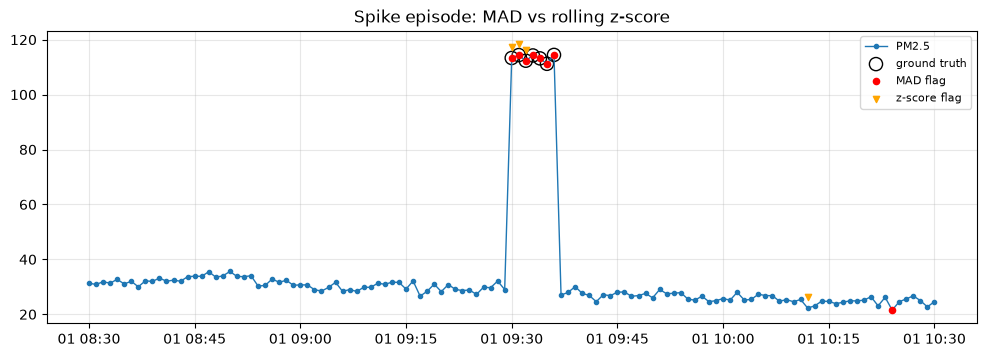
\includegraphics[width=0.9\linewidth]{spike.png}
\caption{One spike episode. MAD flags every anomalous minute; the z-score flags only the first ones (masking).}
\label{fig:spike}
\end{figure}

\textbf{Discussion.} The rolling MAD detector catches every anomalous minute (recall 1.00) and all 32 episodes with no delay. The z-score usually flags only the \emph{first} minute of a spike (Figure~\ref{fig:spike}): once the spike enters the window, it inflates the mean and standard deviation, and the following spike minutes look normal. This is the masking effect also seen in Assignment~3. The median and MAD are not affected while less than half of the window is anomalous.

\textbf{Threshold sensitivity.} The MAD scores saved by the stream were re-thresholded offline (Table~\ref{tab:sens}). F1 rises to 0.97 at $k=5$ and 0.99 at $k=6$ with recall unchanged, because the 71 false positives at $k=4$ are ordinary fluctuations. $k=4$ was fixed before the evaluation. Choosing $k$ from this table would mean tuning on the test labels, so in a real deployment $k$ should be chosen on a separate validation period (here the data suggest $k\approx5$--6).

\begin{table}[H]
\centering\small
\begin{tabular}{@{}cccccc@{}}
\toprule
$k$ & MAD precision & MAD recall & MAD F1 & z recall & z F1 \\
\midrule
3.0 & 0.405 & 1.000 & 0.577 & 0.365 & 0.356 \\
4.0 & 0.787 & 1.000 & 0.881 & 0.236 & 0.366 \\
5.0 & 0.946 & 1.000 & 0.972 & 0.228 & 0.369 \\
6.0 & 0.978 & 1.000 & 0.989 & 0.118 & 0.211 \\
\bottomrule
\end{tabular}
\caption{Threshold sensitivity (computed offline from the stored scores).}
\label{tab:sens}
\end{table}

\section{Real-Time Machine Learning}
\label{sec:ml}
\subsection{Task and features}
The ML component forecasts PM2.5 \textbf{5 minutes ahead} for every sensor. At time $t$ the worker builds nine features from information available at $t$ only:
current PM2.5, 1-minute change, 5-minute change, deviation from the last-15-minute mean, last-15-minute standard deviation, hour of day encoded as $\sin(2\pi h/24)$ and $\cos(2\pi h/24)$ (so that 23:59 and 00:00 are neighbours), current temperature and current wind speed. No feature uses any value after $t$, so there is no leakage.

\subsection{Model and online training}
The model is a linear \texttt{SGDRegressor} with Huber loss (robust to large errors), preceded by a \texttt{StandardScaler}. Both are updated online with \texttt{partial\_fit} in mini-batches of 32. The target is the \emph{change} $\text{pm}_{t+5}-\text{pm}_t$, and the forecast is $\text{pm}_t$ plus the predicted change.

Training follows the \textbf{test-then-train} scheme. At time $t$ the worker makes a forecast and stores it, with its features, in a per-sensor pending queue. Five minutes later the true value arrives: the stored forecast is scored first, and only then is the example added to the training batch. The model therefore never sees a target before predicting it. Examples whose origin or target minute was flagged by the \emph{detector} are not used for training, so spikes do not corrupt the model. This uses the detector's output, not the ground-truth labels, so it is allowed in real time. Each worker has its own model, as a stateful operator would in Flink or Spark.

\subsection{Evaluation}
The first 6 hours are excluded as warm-up, because the model starts untrained. The baseline is \textbf{persistence} (PM2.5 in 5 minutes equals PM2.5 now), which is hard to beat at short horizons. Results are reported on all points and on \emph{normal} points, where neither the forecast origin nor the target minute is an injected anomaly. Spikes and dropouts are sudden and cannot be predicted from the past, so on them the error measures the size of the anomaly rather than forecast quality.

\begin{table}[H]
\centering\small
\begin{tabular}{@{}llcc@{}}
\toprule
Subset & Model & MAE & RMSE \\
\midrule
All points & Online SGD model & \textbf{2.902} & \textbf{9.619} \\
 & Persistence baseline & 3.011 & 10.146 \\
\midrule
Normal points (15{,}459) & Online SGD model & \textbf{1.670} & \textbf{2.182} \\
 & Persistence baseline & 1.763 & 2.206 \\
\bottomrule
\end{tabular}
\caption{Prequential 5-minute-ahead forecast errors ($\mu$g/m$^3$) after the 6-hour warm-up.}
\label{tab:ml}
\end{table}

\begin{figure}[H]
\centering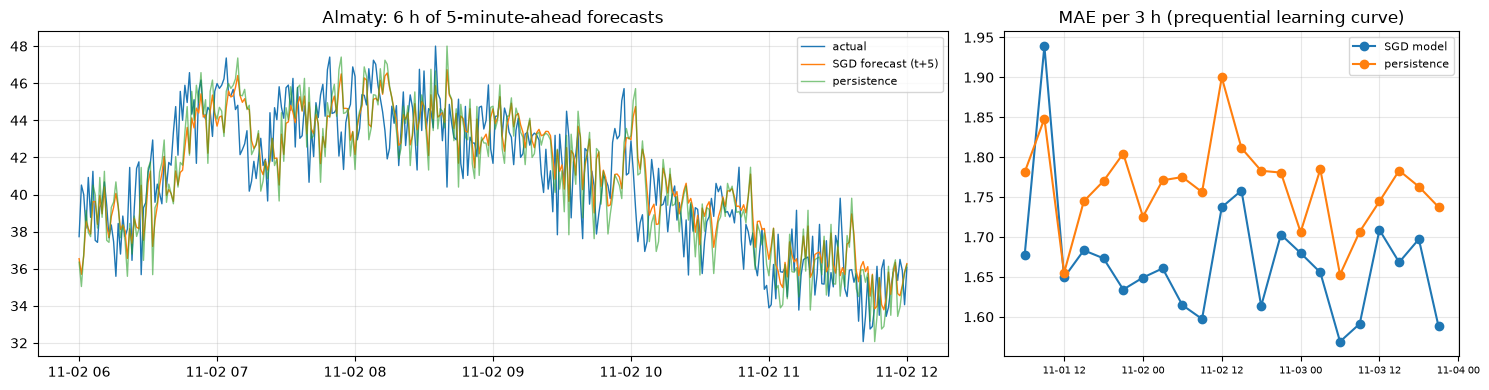
\includegraphics[width=\linewidth]{forecast.png}
\caption{Left: 6 hours of forecasts for Almaty. Right: MAE per 3-hour block (prequential learning curve).}
\label{fig:forecast}
\end{figure}

\textbf{Discussion.} On normal points the online model beats persistence by \textbf{5.3\% MAE} over 15{,}459 truly out-of-sample forecasts. The gain is modest because much of the 1-minute signal is unpredictable noise. The model mainly learns to partly revert noisy jumps towards the recent mean instead of copying them. The learning curve (Figure~\ref{fig:forecast}) shows it ahead of persistence in almost every 3-hour block after the first hours, and it keeps adapting without retraining from scratch. On all points both errors grow a lot (RMSE $\approx10$) because anomalies cannot be forecast. That is why the detector is needed alongside the forecaster.

\section{Operational Characteristics}
\label{sec:ops}
The producer stamps \texttt{t\_ingest} and the worker stamps \texttt{t\_done}, so the end-to-end latency (queueing plus processing) of every event is $t_\text{done}-t_\text{ingest}$. The sink samples the backlog during the run. Table~\ref{tab:ops} summarises the main run (2 workers, 1{,}500 events/s replay rate, live dashboard on).

\begin{table}[H]
\centering\small
\begin{tabular}{@{}lr@{\qquad}lr@{}}
\toprule
Metric & Value & Metric & Value \\
\midrule
Events processed & 17{,}280 & Latency p50 & 2.90 ms \\
Wall time & 11.56 s & Latency p95 & 7.89 ms \\
Throughput & 1{,}494.8 ev/s & Latency p99 & 24.83 ms \\
Backlog mean / max & 3.8 / 50 & Events per worker & 8{,}640 / 8{,}640 \\
\bottomrule
\end{tabular}
\caption{Operational metrics of the main run.}
\label{tab:ops}
\end{table}

\begin{figure}[H]
\centering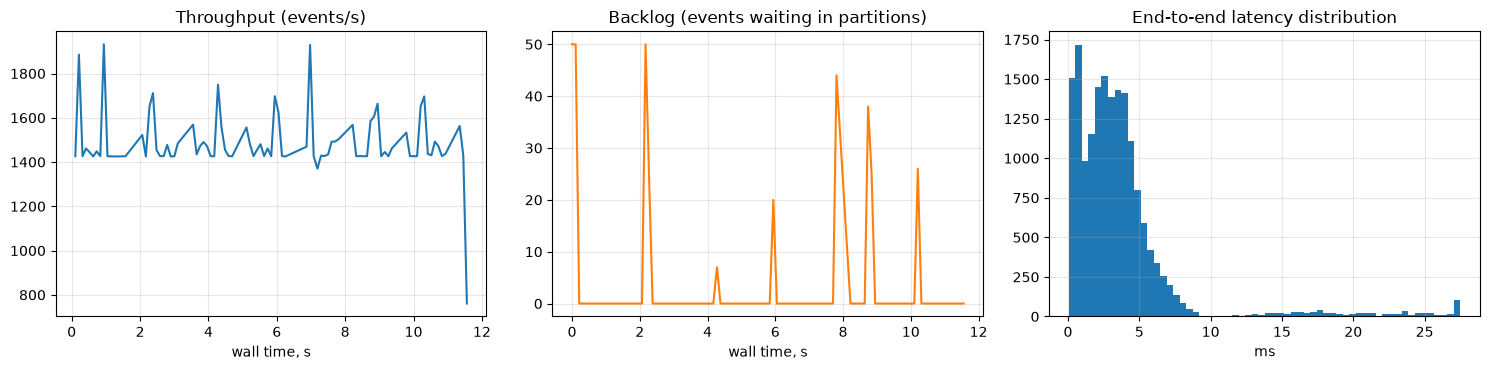
\includegraphics[width=\linewidth]{ops.png}
\caption{Throughput, backlog and the end-to-end latency distribution of the main run.}
\label{fig:ops}
\end{figure}

At 1{,}500 events/s the workers keep up: throughput matches the input rate, the backlog stays near zero and the median latency is a few milliseconds. The p99 outliers coincide with dashboard redraws, which run in the sink thread and briefly hold the interpreter.

\textbf{Scaling experiment.} The pipeline was rerun with 1, 2 and 4 workers and no rate limit (Table~\ref{tab:scaling}). The producer then pushes almost all events into the queues at once, so the backlog climbs to 14--17 thousand events and latency becomes queueing time (hundreds of milliseconds). This is the central streaming trade-off: when the input rate exceeds the processing rate, backlog and latency grow. More threads did \emph{not} raise throughput, because the work is CPU-bound Python and the Global Interpreter Lock lets only one thread run Python code at a time. Real scale-out needs separate processes or machines (a Kafka consumer group, Spark or Flink executors), and the partitioning logic would stay the same. With 4 partitions and only 4 keys, the hash put two sensors in one partition and left another empty ($[0, 4320, 8640, 4320]$). This is \textbf{partition skew}: key hashing balances load only when there are many more keys than partitions.

\begin{table}[H]
\centering\small
\begin{tabular}{@{}clcccc@{}}
\toprule
Workers & Events per partition & Throughput (ev/s) & p50 (ms) & p95 (ms) & Max backlog \\
\midrule
1 & [17280] & 18{,}358 & 431.2 & 805.9 & 14{,}288 \\
2 & [8640, 8640] & 13{,}629 & 563.6 & 1{,}131.8 & 17{,}174 \\
4 & [0, 4320, 8640, 4320] & 15{,}901 & 549.5 & 994.7 & 17{,}150 \\
\bottomrule
\end{tabular}
\caption{Scaling experiment without rate limit (timings depend on the machine).}
\label{tab:scaling}
\end{table}

\section{Limitations and Future Work}
\begin{itemize}\itemsep0pt
\item \textbf{Synthetic data.} Real sensors add missing values, irregular timestamps and calibration drift. The next step is to replay real Astana monitoring data, using the generator only to inject labelled anomalies.
\item \textbf{Threads, not machines.} Because of the GIL, threads do not run CPU work in parallel. The architecture maps directly onto Kafka topic partitions with a consumer group, or onto Spark/Flink keyed streams, where workers are separate processes. Porting the producer to a Kafka client is straightforward.
\item \textbf{Processing time, not event time.} Events arrive in order here. A real deployment needs event-time windows with watermarks to handle late or out-of-order readings.
\item \textbf{Fixed detector baseline.} The 30-minute window reacts slowly to genuine fast level shifts, which are flagged for a few minutes until the window catches up. The threshold should be tuned on a separate validation period.
\item \textbf{Simple model.} A linear model gives a modest gain. Per-sensor models, longer histories or gradient-boosted trees on the same causal features could improve it.
\end{itemize}

\section{Conclusion}
The project delivers a complete, reproducible real-time analytics system for PM2.5 in Astana. A key-partitioned producer/consumer pipeline processes 17{,}280 events at about 1{,}500 events/s with millisecond latency while keeping per-sensor order and state. A live dashboard shows the stream, forecasts, anomalies, throughput and backlog as data arrives. Time-series analysis recovers the daily seasonality (07--08\,h and 18--19\,h peaks) and the upward trend. The rolling MAD detector finds every injected anomaly with zero delay (F1 0.88), while the z-score suffers from masking (F1 0.36). The online SGD forecaster, trained test-then-train on causal features only, beats persistence by 5.3\% MAE. The operational measurements show how backlog and latency explode when the input rate exceeds the processing rate, and why scaling CPU work needs processes or machines rather than threads.

\section*{Reproducibility}
The full implementation, configuration, generated dataset and this report are available at \url{https://github.com/utepbergenoff/realtime_data}.
\begin{verbatim}
git clone https://github.com/utepbergenoff/realtime_data.git
cd realtime_data
python -m venv venv && source venv/bin/activate
pip install -r requirements.txt
jupyter nbconvert --to notebook --execute --inplace main.ipynb
\end{verbatim}
Repository contents: \texttt{main.ipynb} (implementation and results), \texttt{config.json} (all parameters), \texttt{data/astana\_pm25\_stream.csv} (generated stream with ground-truth labels), \texttt{requirements.txt} (dependencies) and \texttt{report/} (this report and its figures).
All parameters are in \texttt{CONFIG}, which is also written to \texttt{config.json}. With \texttt{seed = 42} the dataset (\texttt{data/astana\_pm25\_stream.csv}) is identical on every run. Detection and ML metrics are deterministic for the same data, apart from tiny differences caused by thread scheduling. Timing numbers depend on the machine.

\begin{thebibliography}{9}
\bibitem{kafka} J.~Kreps, N.~Narkhede, J.~Rao. Kafka: a distributed messaging system for log processing. \emph{NetDB Workshop}, 2011.
\bibitem{spark} M.~Zaharia et al. Discretized streams: fault-tolerant streaming computation at scale. \emph{SOSP}, 2013.
\bibitem{flink} P.~Carbone et al. Apache Flink: stream and batch processing in a single engine. \emph{IEEE Data Engineering Bulletin}, 38(4), 2015.
\bibitem{leys} C.~Leys, C.~Ley, O.~Klein, P.~Bernard, L.~Licata. Detecting outliers: do not use standard deviation around the mean, use absolute deviation around the median. \emph{Journal of Experimental Social Psychology}, 49(4), 2013.
\bibitem{gama} J.~Gama, I.~\v{Z}liobait\.{e}, A.~Bifet, M.~Pechenizkiy, A.~Bouchachia. A survey on concept drift adaptation. \emph{ACM Computing Surveys}, 46(4), 2014.
\bibitem{dawid} A.~P.~Dawid. Present position and potential developments: some personal views. Statistical theory: the prequential approach. \emph{Journal of the Royal Statistical Society, Series A}, 147(2), 1984.
\bibitem{sklearn} F.~Pedregosa et al. Scikit-learn: machine learning in Python. \emph{Journal of Machine Learning Research}, 12, 2011.
\end{thebibliography}

\end{document}
